\specialsection{Введение}

\specialsubsection{SMT-формулы}

\underline{SMT-формулы} (от англ. \textit{Satisfiability Modulo Theories}) являются одним из наиболее важных объектов в области практических применений математической логики. Они позволяют сначала формальным образом записать разнообразные утверждения из различных предметных областей, а затем с помощью специальных вычислительных методов проверить логическую выполнимость (состоятельность) этих утверждений.

SMT-формула является некоторым расширением SAT-формулы, которое позволяет использовать не только логические переменные и связки с ними, а ещё и выражения с участием объектов из некоторого домена (например: целые числа, вещественные числа, битовые векторы, массивы) и различными операциями с ними (например: числовая арифметика, битовые операции, взятие элемента массива по индексу и т. д.).

Более формально, SMT-формула является формулой в логике первого порядка, где у каждого символа переменной или функции есть некоторый заранее определенный тип (домен), а в качестве функциональных символов используются функции и операторы из разных доменов (например, те же битовые операции или взятия элемента массива по индексу). Задача проверки выполнимости\footnote{В тексте работы иногда будет появляться выражение <<решение формулы>>, что в данном контексте будет являться синонимом выражения <<проверка выполнимости формулы>>.} такой формулы состоит в том, чтобы выяснить, можно ли для каждой свободной (не находящейся под квантором) переменной подобрать значение соответствующего ей типа так, чтобы при подстановке данных значений формула была истинна. Помимо этого, чаще всего, если формула выполнима, требуется также для каждой свободной переменной выдать значение, сопоставляемое ей. Это отображение из множества свободных переменных в множество их значений называют моделью.

Чтобы стало более понятно, покажу несколько примеров.

Пример формулы:
\begin{equation} \label{smt-example-1}
    (x + y + z = 2) \wedge (x + 2y + 3z = 2) \wedge (x + 2y + 4z = 1),
\end{equation}

где $x$, $y$ и $z$ --- целые числа. Эта формула является выполнимой, поскольку при подстановке значений $x \leftarrow 1$, $y \leftarrow 2$, $z \leftarrow -1$ формула превращается в истинное утверждение.

Ещё пример:
\begin{equation} \label{smt-example-2}
    (x = 2y) \wedge (x = 2z + 1).
\end{equation}

Если потребовать, чтобы $x$, $y$ и $z$ в этой формуле были целыми числами, то формула, очевидно, не будет выполнимой (т. к. в этом случае написанное здесь обозначает высказывание \textit{$x$ является чётным и $x$ является нечётным}). Однако, если разрешить переменным быть вещественными (или хотя бы рациональными), формула станет выполнимой. Этот пример показывает, что свойство выполнимости зависит от типовых (доменных) ограничений, наложенных на переменные и функциональные символы.

Пример формулы с кванторами:
\begin{equation} \label{smt-example-3}
    \exists \ x, y, z: (n \ge 0) \wedge (x > 0) \wedge (y > 0) \wedge (z > 0) \wedge (x^n + y^n = z^n),
\end{equation}

где все переменные являются целыми числами. В этой формуле присутствует только одна свободная переменная --- $n$, поэтому искать подходящее значение нужно только для неё. Нетрудно заметить, что нам подходят значения $n = 1$ и $n = 2$, поэтому формула является выполнимой (но если условие $n \ge 0$ заменить на $n \ge 3$, формула станет невыполнимой согласно Великой теореме Ферма).

Пример формулы с битовыми векторами:
\begin{equation} \label{smt-example-4}
    (x \ge \texttt{\#b01000000}) \wedge (x + (x \ \texttt{shl}\footnote{Здесь $\texttt{shl}$ --- \textit{shift left}: $x \ \texttt{shl} \ y$ есть битовый сдвиг вектора $x$ влево на $y$ битов.} \ \texttt{\#b00000001}) + \texttt{\#b11111111} < \texttt{\#b00100000}),
\end{equation}

где переменная $x$ является битовым вектором размера 8 (фактически, это беззнаковое числом размером 1 байт). Аналогично, все константы\footnote{Вообще константы не принято выносить как отдельную сущность в формулах, поскольку их можно считать функциями от нулевого количества аргументов и, соответственно, обозначать каждую из них своим функциональным символом из логики первого порядка. Но в этой работе для удобства я буду отделять константы, содержащиеся в формулах.} в формуле тоже являются битовыми векторами размера 8 и записываются в бинарном формате. Стоит также отметить, что каждый битовый вектор можно однозначно отождествить с числом через его запись в двоичной системе счисления (например, таким образом происходит сравнение векторов на больше-меньше).

В указанном примере демонстрируется возможность использования переменных, функций и операторов из домена битовых векторов, а также то, что их семантика может отличаться от общепринятых семантик в других доменах. Так, например, все арифметические операции с битовыми векторами (в нашем случае, это два сложения) выполняются с учётом битового переполнения. Из этого, в частности, следует, что формула из примера является выполнимой, т. к. нам подходит значение $x = \texttt{\#b01100000}$ (или 96 в десятичной системе счисления):
\begin{itemize}
    \item $x = \texttt{\#b01100000}$;
    \item $x \ge \texttt{\#b01000000}$ очевидно выполняется;
    \item $x \ \texttt{shl} \ \texttt{\#b00000001} = \texttt{\#b11000000}$;
    \item $x + (x \ \texttt{shl} \ \texttt{\#b00000001}) = \texttt{\#b01100000} + \texttt{\#b11000000} = \texttt{\#b00100000}$ из-за битового переполнения;
    \item $x + (x \ \texttt{shl} \ \texttt{\#b00000001}) + \texttt{\#b11111111} = \texttt{\#b00100000} + \texttt{\#b11111111} = \texttt{\#b00011111}$ опять же из-за переполнения;
    \item $x + (x \ \texttt{shl} \ \texttt{\#b00000001}) + \texttt{\#b11111111} = \texttt{\#b00011111} < \texttt{\#b00100000}$, что и требовалось.
\end{itemize}

% todo: пример с массивами

\specialsubsection{SMT-логики}

Говоря про домены, модальности и типы данных в SMT-формулах, важно рассказать про \underline{SMT-логики} (в русскоязычной литературе их ещё часто называют теориями). Логики задают ограничения на типы переменных, констант, функций и операторов, которые можно использовать в формуле. Согласно языку логики первого порядка, в каждой формуле вне зависимости от теории можно использовать пропозициональные переменные (ложь, истина) и константы, логические связки между ними и кванторы. Возможность использования остальных конструкций уже определяется логикой.

Так, например, логика \texttt{LIA} (\textit{Linear Integer Arithmetic}) позволяет использовать только целочисленные переменные и константы сколь угодно больших по модулю значений, а также арифметические операции и операторы сравнения (больше-меньше-равно) с их участием. Вдобавок, поскольку это линейная арифметика, все термы формулы обязаны быть линейными по каждой из переменных. Примером формулы в такой логике является формула (\ref{smt-example-1}).

Ещё один пример логики --- \texttt{LRA} (\textit{Linear Real Arithmetic}) --- аналог \texttt{LIA}: устроена так же, но позволяет использовать только вещественные переменные и константы (т. е. проверить, решается ли уравнение в целых числах, с помощью этой логики не получится). Здесь уместно вспомнить формулу (\ref{smt-example-2}), которая является выполнимой в логике \texttt{LRA}, но не является выполнимой в логике \texttt{LIA}.

Нелинейные арифметики тоже реализованы в виде логик: \texttt{NIA} (\textit{Non-linear Integer Arithmetic}) и \texttt{NRA} (\textit{Non-linear Real Arithmetic}) во всём похожи на свои линейные аналоги, но не требуют линейности формулы по переменным (формула (\ref{smt-example-3})).

Битовые векторы представлены в логике \texttt{BV} (\textit{Bit Vector}). Эта логика позволяет записывать формулы с битовыми векторами произвольного фиксированного размера, используя битовые (и, или, исключающее или, отрицание, битовые сдвиги и т. д.), структурные (конкатенация двух битовых векторов, вырезание произвольного подотрезка битового вектора, циклические сдвиги и т. д.) и арифметические (сумма, разность, произведение, целочисленное деление, остаток от деления и т. д.) операции с ними, а также операторы сравнения.

Как уже было отмечено, все арифметические операции с битовыми векторами выполняются с учётом битового переполнения, а сравнения на больше-меньше осуществляются через сравнения целых чисел, двоичными записями которых являются сравниваемые векторы. Кроме того, для удобства, каждая арифметическая операция и каждое сравнение есть в двух вариантах: беззнаковом и знаковом. Знаковый вариант отличается тем, что двоичная запись числа (которая порождается битовым вектором) читается не в обычной арифметической семантике, где каждый бит обозначает очередную степень двойки, а в семантике <<дополнение до двух>>, где самая старшая степень двойки учитывается с минусом (именно таким образом хранятся знаковые целые числа в памяти современных компьютеров).

Если говорить про логики, применимые в компьютерных вычислениях, обязательно нужно упомянуть про логику \texttt{FP} (\textit{Floating Point}), которая реализует вычисления с использованием чисел с плавающей точкой. Эта логика похожа на \texttt{BV} тем, что все переменные и константы представляют из себя битовые векторы соответствующих размеров (16, 32, 64, 128 битов), однако отличается тем, что при арифметических операциях и операциях сравнения данные битовые векторы воспринимаются не как двоичная запись целого числа, а как представление числа с плавающей точкой в памяти компьютера согласно стандарту IEEE-754.

% todo: A UF
% ??? Также важной частью являются логики, допускающие использование массивов и неинтерпретируемых функций.

Особое место в списке логик занимают специальные безкванторные логики --- это аналоги обычных логик, в которых запрещено использование любых кванторов существования и всеобщности. Такие логики обозначаются специальным префиксом \texttt{QF\_} (\textit{Quantifier-Free}) в названии (например: \texttt{QF\_LIA}, \texttt{QF\_NRA}, \texttt{QF\_BV} и т. д.).

Чтобы получить более сложные логики, можно объединить две уже существующие. В этом случае, множества допустимых к использованию в формуле объектов и операций объединятся. Например: при объединении логик \texttt{LIA} и \texttt{LRA} получится логика \texttt{LIRA}, при объединении \texttt{QF\_BV} и \texttt{QF\_LIA} получится \texttt{QF\_BVLIA}, при объединении \texttt{LRA} и \texttt{QF\_NRA} получится \texttt{NRA}, а при объединении \texttt{QF\_ABV} и \texttt{QF\_UFBV} получится логика \texttt{QF\_AUFBV}. Некоторые примеры расширения логик схематично изображены на рис.~\ref{smt-logics}.

\begin{figure}[ht]
\begin{center}
    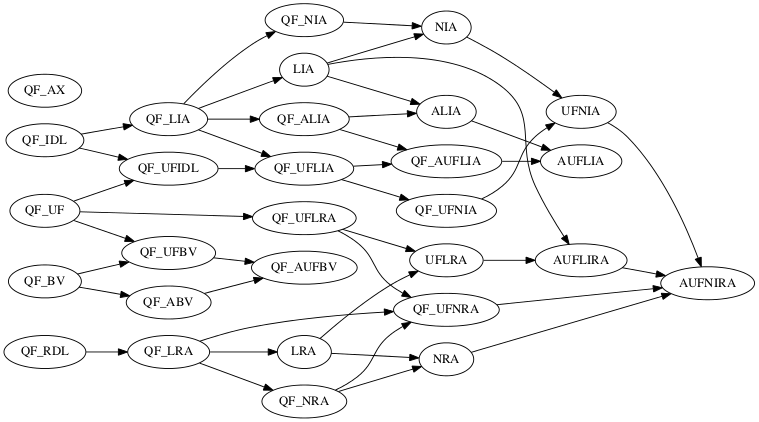
\includegraphics[scale=0.5]{./assets/smt-logics.png}
    \caption{\label{smt-logics} Иерархия, состоящая из некоторых логик, поддерживаемых общепринятым стандартом SMT-LIB \cite{smt-logics-picture}. Если из логики $L_1$ проведена стрелка в логику $L_2$, то $L_1$ является частным случаем $L_2$.}
\end{center}
\end{figure}

Чтобы дополнить список примеров логик напомню, что пропозициональные переменные и константы, а также логические связки между ними по-умолчанию присутствуют в каждой логике. Поэтому существует логика \texttt{BF} (\textit{Boolean Formula}), которая не содержит ничего кроме них, и логика \texttt{QF\_BF} --- её безкванторный аналог. Нетрудно заметить, что решение формул в логике \texttt{QF\_BF} эквивалентно решению задачи SAT.

\specialsubsection{SMT-решатели}

Несмотря на то, что даже самая простая логика \texttt{QF\_BF} уже является NP-полной (т. е. задача решения формул в такой логике является NP-полной), а некоторые логики (например, \texttt{NIA}) являются неразрешимыми, люди всё равно изобретают различные эвристические алгоритмы и прочие подходы к решению задачи проверки выполнимости формул в таких логиках. Комбинации из таких подходов реализуются в специальных программах, называемых \underline{SMT-решателями}\footnote{Или SMT-солверами --- англицизм, также используемый в русском языке.}.

Одним из наиболее известных и, по совместительству, одним из первых из промышленных (т. е. активно используемых как составная часть более сложных программ) SMT-решателей является Z3, разработанный в Microsoft Research \cite{z3-paper}. Он умеет выполнять проверку выполнимости формул и поиск модели, поддерживая самые разнообразные логики.

У Z3 есть конкуренты: решатель cvc5, разработанный в Стэнфордском университете и Университете Айовы \cite{cvc5-paper}, и решатель Yices2, разработанный в исследовательском центре SRI International (Stanford Research Institute) \cite{yices2-paper}. Упомянутые решатели регулярно побеждают Z3 на SMT-COMP, проводимом ежегодно соревновании по решению SMT-формул \cite{smt-comp-paper} \cite{smt-comp-website}, но на практике работают не так стабильно, поэтому реже используются в реальных прикладных задачах.

Ещё одним интересным примером является SMT-решатель Bitwuzla \cite{bitwuzla-paper}, который заточен специально под решение формул с битовыми векторами и без кванторов, поскольку многие практические задачи (например, символьное исполнение) формулируются как раз в таком виде.

Поскольку задача проверки выполнимости формулы является вычислительно сложной, и её решение в большинстве случаев полностью опирается на эвристики, зачастую SMT-решатели не могут выдать никакой ответ для той или иной формулы, даже спустя несколько дней работы. Это может стать существенным препятствием для решения задачи из реальной жизни, которая опирается на подобные формальные методы.

\specialsubsection{Применения}

SMT-формулы обладают достаточно сильной выразительной способностью, поэтому решение многих прикладных задач можно свести к проверке выполнимости и поиску решения для SMT-формулы в некоторой логике.

Среди типовых применений можно выделить планирование задач и составление расписания, вывод типов в языках программирования с зависимыми типами и средства формального вычислительного доказательства теорем, верификация программного и аппаратного обеспечения, статический анализ программ, генерация тестового набора и символьное исполнение. Последнее рассмотрим более подробно.

\specialsubsection{Символьное исполнение}

\underline{Символьное исполнение} --- техника интерпретации программных инструкций, при которой вместо исполнения программы одним конкретным путём, полностью определяемого данными, отправленными программе на вход (т. е. вместо обычного последовательного интерпретирования программных инструкций), программа исполняется сразу всеми возможными путями (при всех возможных комбинациях подаваемых на вход данных). Такой подход был впервые предложен в 76-м году в статье \cite{symbex-intro-paper}.

Проще всего думать про этот процесс так, как будто интерпретатор перебирает все варианты входных данных и на запускает программу на каждом из них, анализируя её поведение. В действительности же такой подход почти невозможно реализовать из-за экспоненциального роста количества вычислений при росте размера входных данных. Поэтому на практике поступают следующим образом:

\begin{enumerate}
    \item Изначально каждой переменной из входных данных сопоставляют некоторое абстрактное значение (такое значение называют символьной переменной).
\end{enumerate}

% todo: дописать пример
% todo: написать про coq и еще че-нибудь

\begin{figure}[ht]
\begin{center}
\begin{minipage}{0.5\textwidth}
\begin{minted}[linenos=true]{cpp}
int foo(int x) {
    int y = x * 2;
    if (y == 24) {
        if (0 < x && x < 20 && x != 12) {
            // this branch is unreachable
            return -1;
        } else {
            fail();
        }
    } else {
        printf("OK");
        return 0;
    }
}
\end{minted}
\caption{\label{symbex-example} Пример программы на языке C.}
\end{minipage}
\end{center}
\end{figure}

\begin{comment}

%New colors defined below
\definecolor{codegreen}{rgb}{0,0.6,0}
\definecolor{codegray}{rgb}{0.5,0.5,0.5}
\definecolor{codepurple}{rgb}{0.58,0,0.82}
\definecolor{backcolor}{rgb}{0.95,0.95,0.92}

%Code listing style named "mystyle"
\lstdefinestyle{mystyle}{
  backgroundcolor=\color{backcolor},
  commentstyle=\color{codegreen},
  keywordstyle=\color{magenta},
  numberstyle=\ttfamily\color{codegray},
  stringstyle=\color{codepurple},
  basicstyle=\ttfamily\small,
  breakatwhitespace=false,         
  breaklines=true,                 
  captionpos=b,                    
  keepspaces=true,                 
  numbers=left,                    
  numbersep=5pt,                  
  showspaces=false,                
  showstringspaces=false,
  showtabs=false,                  
  tabsize=2,
}

\lstset{style=mystyle}

\begin{lstlisting}[language=LLVM, caption=Заголовок]
    call_block:
        %child_hdl = call %coroutine_handle_t g_coro()
        call void @set_child_hdl(ptr %promise, %coroutine_handle_t %child_hdl)
        %suspend_result = call i8 @llvm.coro.suspend(token none, i1 false)
        switch i8 %suspend_result, label %suspend [
            i8 0, label %next_block
            i8 1, label %cleanup
        ]
    next_block:
        %child_promise = call ptr @get_promise(ptr %child_hdl)
        %ret_val = call i32 @get_ret_val(ptr %10)
    \end{lstlisting}

\end{comment}

Такой подход позволяет относительно эффективно искать различные пути исполнения программы и исследовать их: собирать ограничения на входные данные и их инварианты, которые сохраняются в процессе очередного исполнения. В дальнейшем собранные данные можно использовать для задач статического анализа программ, автоматической генерации тестового покрытия, поиска ошибок и уязвимостей в программах.

Одним из популярных инструментов, реализующих такой подход, является символьный движок KLEE \cite{klee-website}, который осуществляет символьное исполнение программ, представленных в виде LLVM-байткода, и используется для генерации тестов и поиска уязвимостей в программном обеспечении \cite{klee-paper}.